%Hierarchy is Chapter > Section > Subsection
%http://www.khirevich.com/latex/ - Tips on Writing a Thesis in LaTeX

\documentclass[a4paper, 11pt, twoside]{report}

\usepackage[activate={true,nocompatibility},final,tracking=true,kerning=true,spacing=true,factor=1100,stretch=10,shrink=10]{microtype}
% activate={true,nocompatibility} - activate protrusion and expansion
% final - enable microtype; use "draft" to disable
% tracking=true, kerning=true, spacing=true - activate these techniques
% factor=1100 - add 10% to the protrusion amount (default is 1000)
% stretch=10, shrink=10 - reduce stretchability/shrinkability (default is 20/20)

\usepackage[T1]{fontenc} %allows for the encoding of unusual or accented characters
\usepackage[bitstream-charter]{mathdesign} %font package similar to the Elsevier font, with included maths style
\usepackage{physics} %provides a family of vector notation

\usepackage{datetime}
\usepackage{graphics} % for pdf, bitmapped graphics files
\usepackage{epsfig} % for postscript graphics files
\usepackage{epstopdf} %nathan tells me I need this one
\usepackage{multirow} %for splitting rows inside tables
\usepackage{float} %for positioning the nomenclature floating tables
\usepackage{color}
\usepackage{subcaption}
\setlength{\parindent}{0em} %don't indent paragraphs
\setlength{\parskip}{1em} %space between paragraphs

%packages that may be useful for formatting
%\usepackage{flushend} %for equalising final page column lengths. messes stuff up sometimes
%\usepackage{setspace}
%\usepackage{pdfpages}
%\hoffset = 9pt
%\voffset = 34pt

\newdateformat{mydate}{\monthname[\THEMONTH] \THEYEAR}
\title{Sensitivity of\\Nozzle Guide Vane Flow Capacity\\to Geometric Changes}
\author{Tom Franklyn Gammage}
\date{\mydate\today}



\begin{document}



\maketitle

\chapter*{Thanks}

\chapter*{Abstract}

\tableofcontents
\listoffigures
\listoftables

\chapter*{Nomenclature}
\subsection*{Romans}
\subsection*{Greeks}
\subsection*{Acronyms and Abbreviations}
\subsection*{Subscripts}



\chapter{Flow capacity - definition and derivation}
%--Include some derivation of how capacity prediction errors can cause exponentially increasing errors in later stages
%--In the relevant chapter, extend capacity to 2D to show how it becomes more nuanced

The capacity of an internal combustion engine is an intuitive concept. It is simple to derive from the engine's geometry, it has tangible units of volume, and it provides an heuristic for the engine's size, performance, and air mass flow rate.

The design of turbomachinery invites an analagous concept to that of IC engine capacity, but a definition is not so obvious. Mass flow rate through an engine's nozzle guide vane is a function of the NGV's geometry and of its boundary conditions. If the mass flow rate can be quantified in a way which mitigates the boundary conditions, then the effects of an NGV's geometry on its mass flow rate may be isolated. A particular NGV will thus have a mass flow rate capacity, just as a particular IC cylinder has a volumetric capacity.

Defining a geometric mass flow rate capacity allows for experimental testing of NGVs without recreating the extreme boundary conditions to which real NGVs are exposed. Setting the correct pressure ratio is sufficent, as the subsequent derivation will show. This expedites the testing of different NGV geometries' effects on capacity.

The predictability of NGV capacity affects the design of every downstream turbine stage. If the NGV mass flow rate differs from its expected value due to a poor prediction, all subsequent turbine stages will be sized for an incorrect mass flow rate. The resulting errors in flow velocity and pressure will compound with each additional stage, leading to increasingly incorrect specification of turbine sizes and turning angles.

Andrea Guiffre' and Matteo Pini~\cite{guiffre_design_guidelines} performed numerical analysis to discuss scaleable guidelines for turbine stage design, validating their model using high-fidelity CFD.  Correct stage matching was found to be highly dependent on matching the \textit{volumetric flow ratio}, defined by the authors as a stage's total-to-static density ratio. To accurately quantify this parameter within the analytical and computational methods discussed in this thesis, flow capacity would need to be predicted correctly.

A strong understanding of capacity predictability should allow engine-makers to pre-empt geometric changes that happen to NGVs during service, such as erosion and cooling hole blockage. It should also account for geometric uncertainties arising from the manufacturing process. While this study advocates for improved accuracy of capacity predictions, emphasis is placed on how these predictions are limited by the unpredictability of real-world manufacture and service.


\section{Mass flow rate through an NGV}

In one dimension, an engine nozzle may be modelled as a compressible flow from an upstream reservoir of total pressure $p_0$, accelerating to velocity $v$ and density $\rho$ through a nozzle of cross-sectional area $A$. Mass flow rate through the nozzle is thus
\begin{equation}
\dot{m} = \rho A v
\end{equation}
where density may be expressed as a function of \textit{pressure ratio}, the ratio of the nozzle pressure to the total pressure
\begin{equation}
\rho = \frac{p_0}{R T_0} \left(\frac{p}{p_0}\right)^\frac{1}{\gamma}
\end{equation}
and velocity is given by the compresssible form of Bernouilli's equation as
\begin{equation}
v = \>
\sqrt[•]{ 
	2 \left( \frac{\gamma}{\gamma - 1} \right) \left[ \frac{p_0}{\rho_0} - \frac{p}{\rho} \right] 
}
\end{equation}

The above equations combine to express mass flow rate through the nozzle as
\begin{equation}
\dot{m} =
A
\frac{p_0}{R T_0}
\left(\frac{p}{p_0}\right)^\frac{1}{\gamma}
\sqrt[•]{ 
2 \left( \frac{\gamma}{\gamma - 1} \right) 
\left[ \frac{p_0}{ \left( \frac{p_0}{R T_0} \right) } - \frac{p}{ \left( \frac{p_0}{R T_0} \right) \left(\frac{p}{p_0}\right)^\frac{1}{\gamma} } \right] 
}
\end{equation}
which simplifies to
\begin{equation}
\dot{m} =
A
\frac{p_0}{R T_0}
\left(\frac{p}{p_0}\right)^\frac{1}{\gamma}
\sqrt[•]{
	2 \left( 
		\frac{\gamma}{\gamma - 1} 
	\right)
	\left[ 
		R T_0 - R T_0 \left( \frac{p}{p_0} \right)^\frac{\gamma-1}{\gamma} 
	\right]
}
\end{equation}
\begin{equation}
\dot{m} =
\frac{p_0}{\sqrt[•]{T_0}} \>
A \;
\sqrt[]{\frac{\gamma}{R}}
\left(
    \frac{p}{p_0}
\right)^\frac{1}{\gamma}
\sqrt[•]{
	\left(
		\frac{2}{\gamma - 1}  
	\right)
	\left[
		1 - \left( \frac{p}{p_0} \right)^\frac{\gamma-1}{\gamma}
	\right] 
}
\end{equation}


\section{NGV capacity in 1 dimension}

Capacity is defined as
\begin{equation}\label{capacity_definition}
\Gamma = \frac{\sqrt[•]{T_0}}{p_0}  \>
\dot{m}
\end{equation}
This provides an expression of mass flow rate independent of upstream total pressure $p_0$ and upstream total temperature $T_0$. The expression is purely a function of throat area $A$ and pressure ratio $\frac{p}{p_0}$:
\begin{equation}
\Gamma =
A \;
\sqrt[]{\frac{\gamma}{R}}
\left(
    \frac{p}{p_0}
\right)^\frac{1}{\gamma}
\sqrt[•]{
	\left(
		\frac{2}{\gamma - 1}  
	\right)
	\left[
		1 - \left( \frac{p}{p_0} \right)^\frac{\gamma-1}{\gamma}
	\right] 
}
\end{equation}
A scale constant $\sigma$ is defined as
\begin{equation}
\sigma = 
\sqrt[]{\frac{2\gamma}{R\left(\gamma-1\right)}} \;
\end{equation}
for a compact expression of capacity as a function of throat area $A$ and pressure ratio $r$:
\begin{equation}
\Gamma \left( A, r \right) = 
\sigma
A \;
\sqrt[]{
	r^\frac{2}{\gamma}
	\left(
		1 - r ^\frac{\gamma-1}{\gamma}
	\right) 
}
\end{equation}
This expression has its maximum value at the critical pressure ratio
\begin{equation}
r_c =
\left(
	\frac{\gamma+1}{2}
\right)
^\frac{\gamma}{1-\gamma}
\end{equation}
At lower ratios, the nozzle is choked and mass flow rate cannot increase further. Choked capacity is given by
\begin{equation}\label{choked_capacity_from_area}
\Gamma_c \left( A \right) =
\sigma
A \;
\sqrt[]{
	\left(
		\frac{\gamma + 1}{2}  
	\right)
	^\frac{2}{1-\gamma}
	-
	\left(
		\frac{\gamma + 1}{2}  
	\right)
	^\frac{1+\gamma}{1-\gamma}
}
\end{equation}

It is shown that the capacity of one-dimensional nozzle flow is a function of only the flow's minimum area, provided the flow is choked and the ratio of specific heats is assumed constant. 

The following chapters will analyse the capacity of two-dimensional and three-dimensional nozzle flows, presenting and discussing analytical techniques for applying the 1D capacity equation to 2D and 3D data. In such cases, capacity will be quantified using equation~\ref{capacity_definition}.

%maybe another paragraph on why this matters for predictability, but maybe this is already appropriate in the chapter intro?



\chapter{Geometric throat area}


% NEEDED DATA:
% -T900 smooth vanes, 6x 2D CFD solutions at various pressure ratios
% -Not sure where the 3D data came from, can we check this? ie --GOM scan data

%plan for chapter - answer the following questions:
% 1) what does "throat area" MEAN beyond 1D? Is it the smallest area across the nozzle, or is it a line/surface drawn according to real flow features, most likely the M1 line?
% 1) why does it work quite well in 2D, ie what is mostly NOT changing between the geometries (could almost say what is incidentally being controlled for)?
% 2) what starts changing in 3D to the extent that no linear signal is recognisable in the noise?

%the raw data consists of: 
% -some 2D vanes with different geometries, and a bunch of 3D vanes with different geometries. Range of PRs. For each, there is a "throat area".
%it is thus possible to plot: 
% -changes in throat area versus changes in capacity for the 2D family, for any given PR
% -changes in throat area versus changes in capacity for the 3D family, for any given PR
% -capacity trends for the 2D and 3D vanes
%for each solution, it is possible to define:
% -a "true throat area" based on the M1 line being crossed at oblique angles by every streamline
% -certain geometric parameters describing how its shape is different to the shape of its other family members

%"throat area" just means the smallest line or surface that can be drawn in a nozzle - not sympathetic to anything actually happening in the flow. It only really works in 1D.

A 1-dimensional supersonic nozzle is equivalent to a single streamline of variable cross-sectional area. It is possible to solve for the flow conditions throughout the nozzle, provided area is specified as a function of position along the nozzle. The mass flow rate capacity is a function of only the flow's minimum area, as in equation~\ref{choked_capacity_from_area}.

A 2-dimensional nozzle may be modelled as a group of adjacent streamlines, each of which may have dissimilar area functions. The streamlines' minimum areas may not correspond to a straight line across the narrowest part of the nozzle. 

This is illustrated in Figure~\ref{fig:illustration_of_minimum_area} by considering the division of a 2-dimensional flow into a finite number of streams of finite width. Each stream has an individual line of minimum width where sonic conditions exist. Collectively these lie on a line distinct from the overall passage line of minimum width. These two definitions of the effective throat line are marked.

If this concept is extended to infinitesimal streamlines (and the flow is isentropic) each streamline will experience sonic conditions at its point of minimum area, combining to form the 2-dimensional sonic line. The effective throat area of a 2-dimensional nozzle is thus the sum of its streamlines' throat areas. This is distinct from the sonic line length, and may be expressed by the integral
\begin{equation}
	\int_{1}^2 \vu*{v} \vdot \vu*{r} dL
\end{equation}
where $\vu*{v}$ is the unit vector of local flow velocity, $\vu*{r}$ is the unit vector perpendicular to the local sonic line, and the integral is performed on the scalar infinitessimal $dL$ over the length of the sonic line, as illustrated in Figure~\ref{fig:illustration_of_equivalent_throat_area_integral}.
 		
%\begin{figure}[H]
%	\centering
%	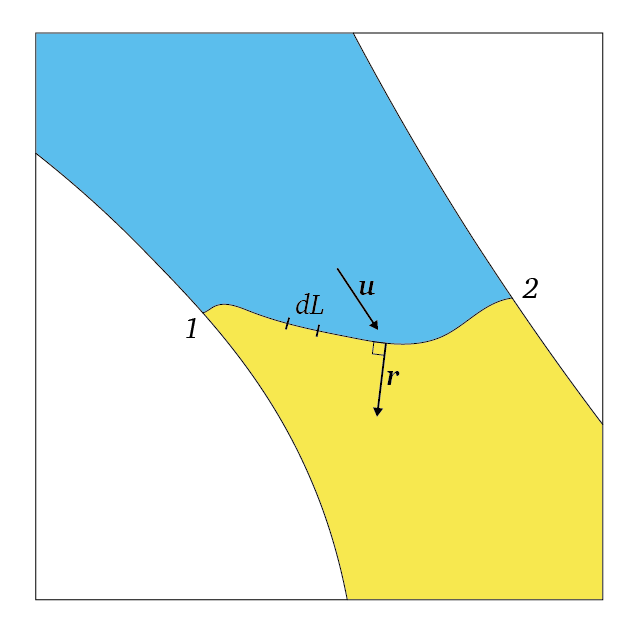
\includegraphics[width=.6\textwidth]{figs/illustration_of_equivalent_throat_area_integral_ver03.png}
%	\caption{Integral for 2D nozzle equivalent throat area}
%	\label{fig:illustration_of_equivalent_throat_area_integral}
%\end{figure}

\begin{figure}[H]
	\centering
	\begin{subfigure}{.45\textwidth}
		\centering
		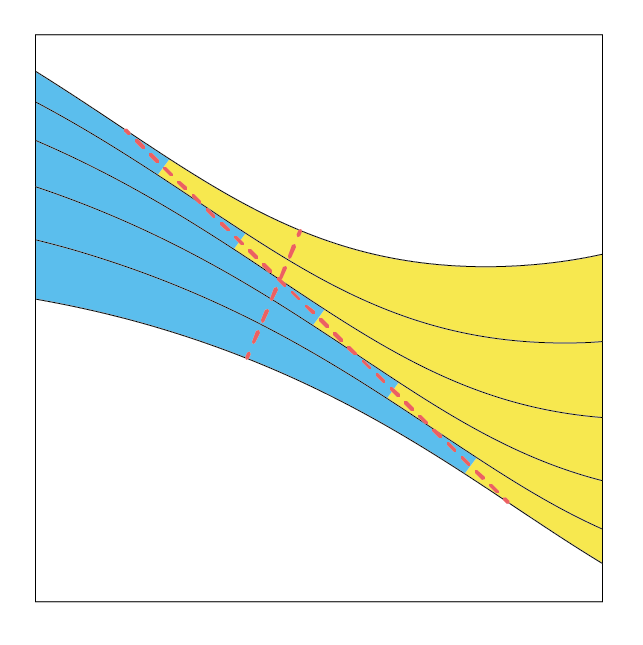
\includegraphics[width=\linewidth]{figs/illustration_of_minimum_area_ver04.png}
		\caption{Different minimum area points of dissimilar streams}
		\label{fig:illustration_of_minimum_area}
	\end{subfigure}
	\hspace{0.05\textwidth}
	\begin{subfigure}{.45\textwidth}
		\centering
		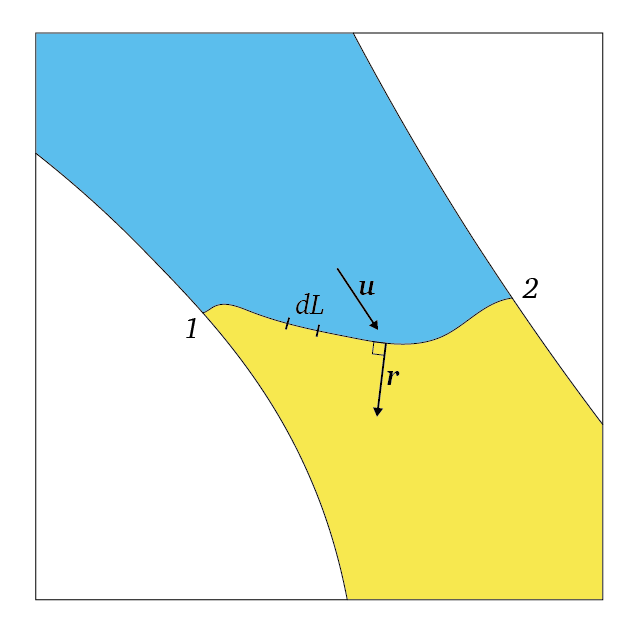
\includegraphics[width=\linewidth]{figs/illustration_of_equivalent_throat_area_integral_ver03.png}
		\caption{Integral for 2D nozzle equivalent throat area}
		\label{fig:illustration_of_equivalent_throat_area_integral}
	\end{subfigure}
	\caption{}
\end{figure}
 		
 --Review any definitions of minimum area from the literature. I haven't got any in the first group of papers from David.


\section{1D vs 2D capacity uncertainty}

-- A family of 2D NGVs were run at various PRs in CFD. The point is to see how their capacity varies when plotted against various definitions of throat area. The usefulness of each definition will be discussed.

-- Present boundary conditions

-- Present mesh

-- When the "throat area" of the 2D family is plotted against their capacity at a choking PR, it shows a pretty good proportional relationship. This is despite some obvious differences in the shape of the M1 line.

-- Why are there still small deviations? That is, can I present a better definition of throat area that fits even better? Possible topics:

 -- Most likely it will follow the 1D rule if it is taken to be that streamline's M1 point. But not certain.
 
 -- the relationship between the minA line and the M1 line
 
 -- the total length of each M1 line
 
 -- a plot of capacity vs M1 line length

-- Why aren't there larger deviations? That is, can I derive a sensible geometric parameter and show that it isn't changing significantly?

-- Is this all really at design PR? What if the M1 lines were obtained at more choked PRs but I forgot to say so? What does the correlation look like at other PRs?


\section{2D vs 3D capacity uncertainty}

-- 3D CFD data was shared by Rolls-Royce for comparison with the 2D data. The point is to see why 3D is still so different from 2D, ie what are we failing so badly to predict with 2D?

-- Discuss the most important ways in which the 3D capacity trends are different from the 2D ones. From a superficial look it appears that the 3D trends never choke. What could this mean about their having a M1 line at all?

-- What does the correlation look like at other PRs?

-- Review 3D effects from the literature.



\chapter{Trailing edge}
%How the trailing edge can drive capacity changes (and loss changes incidentally). These changes are discussed as those happening in-life to the existing engine parts, and also those resulting from an alternative design.
%Why am I including "loss" here, when this part is really about the robustness of capacity predictions on vanes that will change shape with wear? Because the proposed alternative design needs to be decent for loss to be a viable alternative.

%NEEDED DATA:
%-SS cutbacks, all solutions
%-PS cutbacks, all solutions
%-variable cooling rate CFD
%-Larger pictures of the different meshes used
%-Larger contour plots for the different levels of TE SS erosion
%-MinA and M1 lines for the TE SS cutbacks  
%-"Rolls-Royce vs this study" geometry illustration should be remade to be at the same angle as all the flow pictures

%Plan for chapter - answer the following questions:
%1) How does erosion to the SS flange alter 2D mid-span capacity, and which mechanism best explains the changes?
%2) According to the literature, would a 3D investigation into this be justified?
%3) How capacity-predicable would an altrernative design of TE be?
%4) Would said alternative design reduce "loss"?


\section{Definitions of loss for trailing edge performance evaluation}
%--How does it perform in terms of loss?
%--First review the literature to decide what is "loss".

Loss may refer to any process whereby the recoverable energy of a turbomachinery flow is reduced during transit through a turbine stage, other than by shaft work, with corresponding entropy creation. Minimisation of loss remains a primary obective of turbomachinery design, but there is not a universal consensus on how to quantify it.

Daniel Back da Trinidade et al~\cite{trinidade_loss} characterised sources of loss as shock loss, profile losses, tip leakage, endwall losses, and cooling losses. Tip leakage results from flow through the clearance space between the vane tips and the casing. It will not be considered by the present study, since the present study is of fixed NGVs. Endwall losses result from 3-dimensional secondary flows, and will not be considered in the present study which is of 2-dimensional phenomena.

Trinidade et al characterised shock loss as resulting from entropy creation across the shock wave during supersonic flow. The present study will consider this mechanism during discussion of CFD results at choking pressure ratios.

Profile loss was characterised by entropy creation by viscosity in the boundary layer on the blade surface. Entropy generated near the blade's trailing edge was considered as profile loss due to the high entropy creation in the wake region following flow separation at the trailing edge. The authors extended this definition to include the entropy generated as the flow turns tightly around the trailing edge curvature and forms expansion waves.

The authors also defined the category of cooling losses to refer to the aerodynamic penalties incurred by cooling in general, namely ``thicker blade profiles from coolant holes, interaction of coolant film with the blade boundary layer, mixing losses between coolant and main flow and endwall losses.'' The present study seeks to isolate the mechanisms whereby film cooling causes boundary layer changes and mixing effects, discussing film cooling in Chapter~\ref{chapter_leading_edge}.

The present study seeks to define a coefficient of NGV total pressure loss whose arguments are flow measurements or numerically predicted parameters. Giel et al surveyed the total pressure wake profiles of a blade at mid-span, defining a \textit{total pressure coefficient} as
\begin{equation}
Cp_t = \frac{
p_{01} - p_{02}
}{
p_{01} - p_2
}
\end{equation}
where $p_{01}$ and $p_{02}$ are the inlet and wake total pressures, and $p_2$ is the wake static pressure. This definition is to be used for the total pressure wake profiles in this thesis. The authors also defined a \textit{kinetic energy loss coefficient} as
\begin{equation}
e_2 = \frac{ 
\left( \frac{p_{01}}{p_{02}} \right)^\frac{\gamma-1}{ \gamma } - 1 
}{
\left( \frac{p_{01}}{p_{2}} \right)^\frac{\gamma-1}{ \gamma } - 1 
}
\end{equation}
Giel et al's results will be compared to those of this study, considering wake profiles and loss as a function of trailing edge thickness.

Jie Gao et al~\cite{gao_te} defined a slightly different \textit{total pressure loss coefficient} as
\begin{equation}
C_pt = \frac{
p_{01} - p_{02}
}{
p_{02} - p_2
}
\end{equation}

--Discuss these two slightly different definitions


 
--Saha paper has its own loss definitions too - seems to be doing a definition that considers the coolant/mainstream mass flow ratio.
\begin{equation}
\zeta = 
1 -
\frac{ 
	\left( 1 + Y \right) 
	\left(
		1 -
		\left(
			\frac{p_2}{p_{02}}
		\right)
		^\frac{\gamma-1}{\gamma}
	\right)
}{
	\left(
		1 -
		\left(
			\frac{p_2}{p_{01}}
		\right)
		^\frac{\gamma-1}{\gamma}
	\right)
	+Y
	\left(
		1 -
		\left(
			\frac{p_2}{p_{0c}}
		\right)
		^\frac{\gamma-1}{\gamma}
	\right)
}
\end{equation}
where $Y$ is the coolant-to-mainstream mass flux ratio.


\section{Effects of trailing edge shape uncertainty on capacity predictability}

--Uncertainties in the trailing edge shape (SS erosion and manufacturing variations) - how hard do they make it to predict capacity

-- Uncertanties occur in the suction-side traling edge because of various factors like erosion through cooling failure (for example in desert environments) and manufacturing variations. If variations and life-cycle changes happen to the trailing edge, what effect on capacity can we expect, and why?

--Review the literature on what sort of erosion is expected, and show that it’s justified to look at a 2D midspan slice as I have done, because this the hottest bit of the part and more erosion would happen here anyway.

--2D CFD was run for 1 NGV with varying amounts of erosion simulated on the TE SS flange.

--Present boundary conditions

--Present mesh with larger and better pictures, and show how the mesh is altered as erosion amount varies

--Show capacity trend for all the data as an initial summary, then show capacity vs erosion amount for a couple of relevant PRs (perhaps design and fully choked)

--2D CFD predicts a maximum ~2 percent change in capacity (when the flange is completely gone)

--What is changing in the flow as a result of the erosion, and is it driving capacity change via the expected route of throat area changes (whatever we've decided is the best definition of throat area in the previous chapter)

--Cite the state of the art for measuring the capacity of a ring of real parts - Burdett:
	--Daniel Burdett - Analysis of ultra-low uncertainty gas turbine flow capacity measurement techniques~\cite{burdett_capacity_measurement}
		--Arguing: Experimental capacity measurement of a ring of NGVs is now excellent and getting better. CFD still has trouble with small geometric changes because they are so tiny compared with even small deviations in the mesh. The TE is especially difficult to model with CFD because it involves so many different flows meeting and mixing, with unpredictable geometry
		--Raw data: Experimental data showing continued improvements to the accuracy of the unsteady capacity measurement technique
		--I discuss: The TE is indeed particularly hard to predict. Having established an extremely accurate measurement technique for an annulus of NGVs, how could such ideas be adapted to focussing on small geometric changes at the TE?
		--I also cite: The history of this technique at Oxford, showing it has embodied a continual evolution in measurement accuracy and sensitivity to boundary conditions, but has been relatively underused for the study of geometric effects
		
--Jie Gao - Experimental and numerical investigations of trailing edge injection in a transonic turbine cascade~\cite{gao_te}
	--Arguing: TE coolant ejection is good for reducing the wake size and reducing shock effects on the exit angle
	--Raw data: Their experimental and CFD linear cascade, five-hole probe data and surface pressure plots, downstream loss profile
	--I discuss: Does it match my blowing rate study? Do my turning angles agree with theirs as Mach number changes? Do I see the same reduction of shocks? Do I broadly agree about the benefits of TE ejection? Remember badly-predicted turning angles are like bad capacity predictions
	--I also cite: Whoever's loss definition they use - why didn't they compare it to others?
	--My raw data: A lot of my own TE CFD
	
Gao et al experimentally and numerically investigated the external flow field near the trailing edge of a linear cascade with trailing edge injection. The authors' focus was on the effects of the trailing edge coolant flow on the vane's loss mechanisms and flow exit angle. Without trailing edge injection, increased exit isentropic Mach number caused the appearance of trailing edge suction side shock waves which altered the flow angle. With trailing edge injection, there was a slight reduction in this shock effect but a strong reduction in the shock wave near the trailing edge pressure side.
		
		
\section{Performance of an alternative trailing edge design}
%--Centred-ejection option (PS cutbacks) (and could it reduce loss) and what happens as its geometry is changed to gradually look more like an existing design
%--We must also consider broader TE manufacturing changes that are likely to happen on purpose - the switch to CMC manufacturing of turbine blades. How will this change the game, and what tolerances are expected?

Improved materials and manufacturing techniques may neccessitate alternative trailing edge geometries. Paul W. Giel et al~\cite{giel_te_thickness} noted that ``in the pursuit of higher turbine inlet temperatures for reduced fuel burn and emissions consistent with NASA's goals~\cite{giel_nasa_reference}, Ceramic Matrix Composite (CMC) materials are now being implemented in gas turbine engines...They enable higher turbine inlet temperatures, thus enabling higher overall pressure ratios (OPRs) for the engine and higher thermal efficiency.'' 

The authors used a linear cascade to measure the aerodynamic performance of a set of blades representing the geometric constraints of the CMC manufacturing method. Of main concern was the constraint that ``the trailing edge thicknesses of CMC blades are anticipated to be significantly larger than those of current state-of-the-art metallic blades,'' which may be expected to cause increased loss. 

--discuss other justifications for studying this design - is it more predictable because it suffers less erosion?

--Introduce my alternative design: 2D CFD was done on an alternative design of TE featuring centred coolant ejection. This shape of TE was also incrementally cut back on the pressure side so as to more resemble the existing TE design.

--Present boundary conditions

--Present mesh with larger and better pictures, and show how the mesh is altered as the design is altered

--Plot capacity trends for the centred-ejection designs vs the baseline

--Is there better capacity predictability because the effects of erosion are less pronounced due to the thicker flanges?

--Discuss whether this loss may be worse or better if a centred-ejection design is used, still perhaps plotting more than one definition of loss

--When using this configuration, is there an optimal blowing rate that might re-energise the base region? Plot blowing rate vs loss, remembering that the graph I currently have is erroneously for the other type of TE, not for the centred-ejection kind. Should I try to re-run just this one thing?

--Compare my centred-ejection TE with a "naturally-formed by erosion" centred-ejection TE from the literature 


 
 


To be filed:

--Ranjan Saha - SHOWER HEAD AND TRAILING EDGE COOLING INFLUENCE ON TRANSONIC VANE AERO PERFORMANCE~\cite{saha_loss}
	--Arguing: Loss turns out very differently depending on which loss equation you use, and some formulations might be better than others
	--Raw data: Their annular sector rig which tested NGVs with and without showerhead and TE coolant to quantify loss
	--I discuss: How do their definitions of loss compare to mine and others', and is there an answer to which one is best in general?
	--I also cite: All the other possible loss definitions, going back to Raffel and Kost and further if necessary
	--My raw data: Any of my CFD data can yield loss according to any preferred definition, but this is most pertinent to my T900 TE cutbacks discussion





\chapter{Leading edge}
\label{chapter_leading_edge}
%How the LE matters too.

%NEEDED DATA:
%-XWB 84K SS cooling hole 2D CFD solutions - not sure if there are multiple PRs converged, can we check that?
%-XWB 84K SS cooling hole quasi-3D solutions - again not sure about other PRs
%-More detailed and extensive surface pressure plots of the XWB CFD
%-Surveys of total and static pressure across the passage at or shortly before the throat, to see how it changes with the hole moving
%-Plot of how coolant TP compares to mainstream TP at each different injection point - this could all be compared to Hambidge's analytical work on capacitty and coolant ejection
%-More illustative contour plots showing any differences between the two turbulence models

%Plan for chapter - answer the following questions:
%1) How is capacity affected by where exactly additional film coolant is introduced?
%2) What current models best explain the effects of film coolant row location on capacity?
%3) What corrections are necessary to interpret these 2D slot results in the real context of 2 rows of holes?

--It is sometimes necessary to add extra cooling holes on the suction-side at the LE

--Coolant introduced into this part of the flow has complex interactions with the mainstream, affecting NGV capacity
 
 
\section{sensitivity of capacity to cooling holes on the leading suction side}

--Adding cooling holes causes complex effects - here discussed as loss, so I need citations for capacity too:
--Jie Gao - Experimental and numerical investigations of hole injection on the suction side throat of transonic turbine vanes in a cascade with trailing edge injection~\cite{gao_te_and_film_cooling}
		--Arguing: Like their above paper but with a SS cooling slot. It causes passage blockage, a thicker wake, and more loss. But when there are shock waves, the film coolant enhances the TE PS shock but reduces the TE SS shock, which could be used toreatly reduce the TE SS shock if the injection is upstream of the throat
		--Raw data: Their experimental and CFD linear cascade, with strong emphasis placed on the loss definitions and techniques established by Denton and Xu, Mee et al, and Schobieri
		--I discuss: Ways in which my SS injection might interact with the flow (including shockwaves) as they suggest. Will I see it without having TE injection too?
		--I also cite: Denton and Xu, Mee et al, and Schobieri for established precident on loss quantification
		--My raw data: My moving coolant row study

--2D CFD was done on an XWB NGV with no coolant features apart from the addition of a single cooling row on the upstream suction side. The position of this featrure was varied, thus varying whereabouts in the flow the coolant was introduced.

--Present boundary conditions

--Present mesh, showing how the variable location coolant row is introduced

--Review the literature for why correctly modelling turbulence is important for capturing the mainstream/coolant mixing, and thus why two turbulence models are compared.

--Plot capacity changes versus hole position and discuss its causes, mentioning the literature reviewed in the chapter intro (plus the two definitions of capacity where coolant is concerned - which one is used in earlier chapters??) A maximum ~0.5 percent change in capacity resulted from an unrealistically drastic shifting of a 2D cooling slot along the vane's suction side.

    
\section{Consideration of corrections necessary to interpret 2D result}

--Different:

--Mass flow rate between a 2D slot and a 3D row of holes

--Mixing between coolant and mainstream

--Angle of ejection

--Papers about matching the conditions when simulating a cooling row:

--S. Ravelli - NUMERICAL ASSESSMENT OF DENSITY RATIO AND MAINSTREAM TURBULENCE EFFECTS ON LEADING EDGE FILM COOLING: HEAT AND MASS TRANSFER METHODS~\cite{ravelli_engine_conditions}
		--Arguing: In a CFD simulation of four film cooling hole rows, the usual parameters (DR, BR, MFR, TuI) aren't enough to ensure you have matched the engine conditions
		--Raw data: A previous experimental study (PSP) to validate their CFD, and their CFD
		--I discuss: Criticise my own signle cooling slot work - is it really representative enough for its capacity effects to be predictable
		--I also cite: Other CFD on film cooling
		--My raw data: My single cooling row data, emphasis on the CFD parameters and setup
		
--Giovanna Barigozzi - Experimental investigation of the interaction between showerhead coolant jets and main flow~\cite{barigozzi_film_cooling}
		--Arguing: When film coolant is ejected upstream , observed high turbulence and velocity fluctuations suggest the mixing is a random process without coherent structures, and unsteady, and 3D
		--Raw data: Their experimental study, including pressure-sensitive paint and particle-image velocimetry
		--I discuss: Do we know less than we thought about how much film coolant is actually getting to the LE SS? Reason why you might want an extra row there? Also, clear support for my arguing that proper CFD investigations of SS LE film cooling should not be a 2D slot and should not be steady
		
--Wei He - Film cooling and aerodynamic performances of a turbine nozzle guide vane with trenched cooling holes~\cite{he_film_cooling}
		--Arguing: A novel design for film cooling holes, using a zigzag-shaped trench, has some advantages but is only really suitable for the middle PS
		--Raw data: Their 3D CFD on a single-vane linear cascade, where the trench moves around various positions
		--I discuss: They mention BR etc, relevant to me. Their movable trench is a bit like my movable 2D slot, except it is mainly confined to the PS, whereas mine is on the SS. But my quasi-3D study could be easily adapted to repeat their study of the novel trench shape
		--My raw data: My Q3D study



\addcontentsline{toc}{chapter}{Bibliography}
\bibliographystyle{ieeetr}
\bibliography{tmfg_bibliography_ver01}



\end{document}